\documentclass[titlepage,landscape]{seminar}
\usepackage{url}
\usepackage{graphicx}
\usepackage[pdftex]{color}
\usepackage{hyperref}
\usepackage{epstopdf}
\usepackage{slides}

\begin{document}

\myslide{
\begin{center}
\begin{tabular}{lccc}
\hline\hline
Taxon & $4N_e\mu$ & $4N_e\mu$ (low coverage) & $\epsilon$ \\
\hline
{\it Cionia intestinalis} & 0.0111 & 0.012 & 0.00113 \\
{\it Daphnia pulex} & 0.0011 & 0.0012 & 0.00121 \\
\hline
\end{tabular}
\end{center}
}

\begin{center}
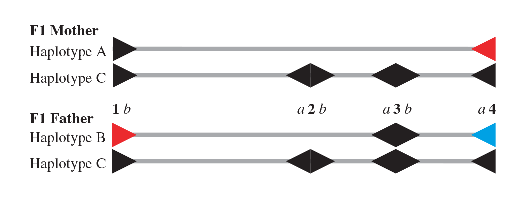
\includegraphics[width=0.9\textwidth]{RAD-heterozygosity.eps}
\end{center}

\begin{center}
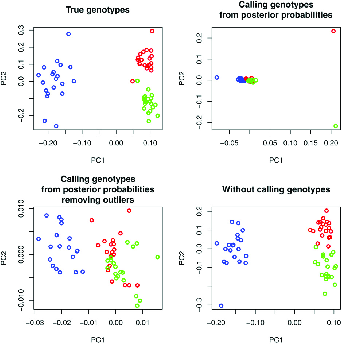
\includegraphics[width=0.8\textwidth]{fumagalli-PCA.eps}
\end{center}

\myslide{
\begin{itemize}

\item 2039 individuals with four grandparents born within 80km of one
  another, effectively studying alleles sampled from grandparents
  (ca. 1885). 

\item 6209 samples from 10 countries in continental Europe.

\item Autosomal SNPs genotyped in both samples~(ca. 500K). 

\end{itemize}
}

\myslide{
\begin{itemize}

\item Average pairwise $F_{ST}$: 0.0007

\item Maximum pairwise $F_{ST}$: 0.003

\end{itemize}
}

\begin{figure}
\begin{center}
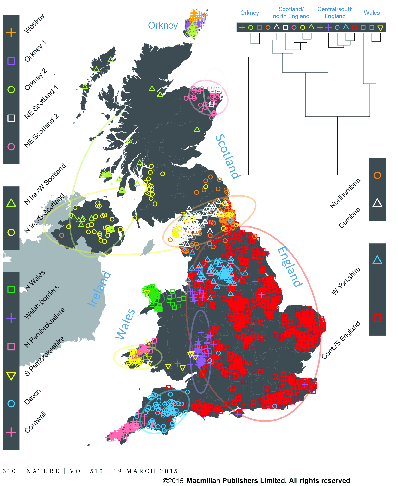
\includegraphics[height=0.9\textheight]{fine-structure-britain.eps}
\end{center}
\caption{{\tt fineSTRUCTURE} analysis of genotypes from Great Britain.}
\end{figure}

\begin{figure}
\begin{center}
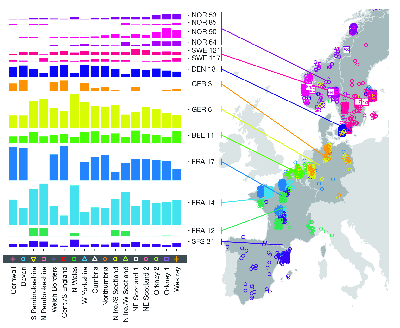
\includegraphics[width=0.8\textwidth]{UK-Europe.eps}
\end{center}
\caption{European ancestry of the 17 clusters identified in the UK.}\label{fig:UK-Europe}
\end{figure}

\end{document}
